\chapter{Blockchain Download}\label{section-blockchain-download}
This section will cover the approach taken to retrieve and store all historical Bitcoin transactions, up to an appropriate (recent) block height of 570,000 - mined on 3rd April 2019. 

\section{Hardware}\label{satoshi-specs}
I had access to a VM on a machine provided by the Department of Computing at Imperial.  My VM has the following resource allocated to it:
\begin{itemize}
    \item \textbf{Processor}: 16 of 24 cores, AMD EPYC 7401
    \item \textbf{Memory}: 16GB
    \item \textbf{Storage}: $\sim$5TB SSD Available
\end{itemize}

\section{Retrieving historical Bitcoin Transactions}
After analysing the various approaches taken previously to retrieve all bitcoin transactions, I decided to adapt the contribution of Max Baylis' Health Monitoring project [see \ref{background-max-baylist-project}]. Max's approach uses WebFlux to create parallel streams of data fetched using RPC and writes it to MongoDB; I adapted this work to divert the data into a CSV format suitable for importing into Neo4J. Below we describe the steps taken to successfully build CSV files for the entire Bitcoin Blockchain. 

\begin{itemize}
    \item Introduced a new API endpoint. The new endpoint was named \texttt{extractBitcoinToNeo4j}. This accepted two arguments as path variables, \texttt{fromHeight} and \texttt{toHeight} which are to be used to define the range of blocks to fetch data from. 
    \item Using the parameters \texttt{fromHeight} and \texttt{toHeight}, I then generate a Flux stream which uses RPC to invoke the method \texttt{getBlockHash} on a \textit{bitcoind} \ref{background:bitcoind} instance running in a container on the same machine. 
    \item The Flux stream of block hashes are then mapped to the actual block data using flux's \texttt{flatMap} operation and by invoking the method \texttt{getBlock}, passing it the block hash from the previous step. 
    \item The block data is retrieved and deserialised to an intermediary representation in Java. Each block is then appended to a CSV file in the format required for an import into Neo4J. 
    \item The retrieval of a single block will then initiate the process of fetching transactions; the Flux of blocks will be mapped to individual transactions by fetching each of the transaction ID's in the block and again using RPC to invoke the \texttt{getrawtransaction} on the \textit{bitcoind} instance in order to fetch all the data for each transaction. 
    \item Each retrieved transaction will be written to CSV, in addition to writing the relationships between transactions, blocks and outputs to their own CSV files. 
\end{itemize}

\begin{figure}[h!]
  \centering
  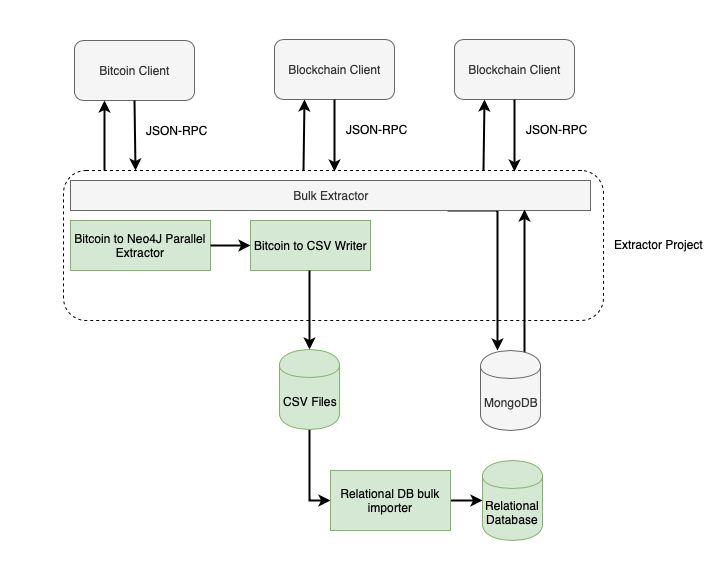
\includegraphics[width = 15cm]{./figures/adding-bitcoin-extractor-diagram}\\[0.5cm] 
  \caption{A architecture diagram displaying the new components (in green) I introduced to Max's Blockchain Health project while implementing Bitcoin to Neo4J historic data population}
  \label{fig:neo4j-layout}
\end{figure}

\section{Challenges \& Solutions:}
\subsection{Efficiency}
With multiple cores at my disposal, it would only be logical to try and distribute the workload across the cores. Fortunately, WebFlux conveniently provides functionality to do this; by adding \texttt{.parallel(n)} to my Flux stream, the workload is divided up into \texttt{n} rails (a rail is a subset of the work to do). Then subsequently applying the \texttt{.runOn(Schedulers.parallel())} mapping, WebFlux is told to parallelise this work by running each rail on a separate core. 
\subsection{Job failure mitigation}
When an error from the client is received, possibly due to being overwhelmed with requests or a temporary network issue, it would be an inefficient and a naive approach to allow a single failure to cause the entire job to fail. Therefore I mitigated job failure by adding retry logic to RPC requests, so that failures will first be handled by initiating a re-try mechanism with a delay (the delay necessary to allow time for recovery in the case of being overwhelmed). However, if an unexpected error occurs that we have not anticipated, the entire job may fail. Therefore, when performing the download, I ensured to do so in incremental batches. Specifically, we first download data for blocks 0-100,000 then 100,001-200,000 and so on. Therefore, if a failure does occur, progress from other blocks has been saved from previously successful runs and only the batch which failed needs to be re-run. 

\subsection{Writing concurrently from several threads}
Although the above parallelisation improves the efficiency of the overall download process, it introduced the problem of multiple threads writing to a single CSV file concurrently, which led to data in the CSV files being malformed where threads have written data chunks in an interleaving fashion. 

\subsubsection{Fix interleaving writes with a lock} 
Clearly each line in the file needs to be written atomically, so I introduced a lock that each thread must hold in order to perform a write to a CSV file. However, I quickly realised that this will create a significant bottleneck in the workflow and developed an alternative solution.

\subsubsection{Fix interleaving writes with per thread files} 
To enable parallel file writing and circumvent the bottleneck of acquiring locks, we enabled each thread to write to a separate file. For example, the CSV file containing the block nodes will be named \texttt{block-data-thread-1.csv}, \texttt{block-data-thread-2.csv} and \texttt{block-data-thread-3.csv} when created by threads with id's 1, 2 and 3 respectively. With this solution, each write can occur without risk of another thread also attempting to write, so the necessity to acquire a lock for concurrent access no longer exists. 

\subsection{Duplicate Addresses}
While generating the CSV files, we fetch the outputs of a transaction and the addresses each output is locked to. While generating the CSV, there was no way of efficiently checking if we had already seen an address before, we simply had to write every address we see to the CSV file. Consequentially, when running the Neo4J bulk import job, we encounter an error as we attempt to define an address node twice. A solution considered was to use a flag \texttt{--ignore-duplicate-nodes} that can be used when invoking the bulk import tool. This would simply ignore any address nodes that have already been defined, solving our problem. However, as TokenAnalyst found in their work \cite{RefWorks:doc:5c98e0cde4b044512c0b8641}, the \texttt{--ignore-duplicate-nodes} flag massively slows down the import process, as Neo4J needs to check every single node to see if the one its adding already exists. Their solution, which I adopted, was to use GNU's \texttt{sort - u} command, which allows us to generate a new address CSV file with only the unique addresses. TokenAnalyst found this process to take around 30 minutes \cite{RefWorks:doc:5c98e0cde4b044512c0b8641}, and is therefore a good investment in speeding up the entire import process. 


\subsection{Result}
All Bitcoin Blockchain data was able to be downloaded, parsed and written as CSV files across a 12 hour period up to block 570,000. Due to the process of human intervention in my approach, in order to mitigate the effects of a job failing as described above, the download was not continuous and there were idle times between jobs finishing and the next being started. Additionally, manual intervention was required post-download in order to augment the Bitcoin data with price information and entity relationships, as described in section \ref{section-price-data} and section \ref{section-entity-tagging} respectively. 